\documentclass{book}
\usepackage[utf8]{inputenc}
\usepackage[english,ngerman]{babel}
\usepackage{datetime}
\usepackage{graphicx}
\usepackage{xspace}
\usepackage{hyperref}
\usepackage{listings}
\usepackage{float}
\usepackage{keystroke}


\newdateformat{germanDate}{\twodigit{\THEDAY}.\twodigit{\THEMONTH}.\THEYEAR}

% eigene Commands
\newcommand{\sketchup}{\texttt{SketchUp}\xspace}
\newcommand{\rubyXL}{\texttt{rubyXL}\xspace}
\newcommand{\inifile}{\texttt{inifile}\xspace}
\newcommand{\robersexcelconvert}{\texttt{RobersExcelConvert}\xspace}

%\setcounter{secnumdepth}{0}
\begin{document}
	
	\begin{titlepage}
	\centering
	
\includegraphics{pics/sketchup-icon}\par\vspace{1cm}
	%		{\scshape\LARGE Columbidae University \par}
	
	\vspace{1.5cm}
	{\huge\bfseries Robers' Excel Convert\par}
	\vspace{1cm}
	{\scshape\Large - Anleitung -\par}
	\vspace{2cm}
	{\Large\itshape Timo Bergerbusch\par}
	\vfill
	im Auftrag von:\par
	Max Robers
	
	\vfill
	
	{\large \germanDate\today\par}
\end{titlepage}
	
	\tableofcontents
	\chapter{Einleitung}
	
	\chapter{RobersExcelConvert}
	\chapter{Voraussetzungen}
		\section{\sketchup Version}
			Die \sketchup-Version, welche benötigt wird ist bei derzeitigem Wissenstand nur die 2018-er Version. Es wird eine solche moderne Version benötigt, da ältere \sketchup-Versionen, wie zum Beispiel die 2015 Version die eingebaute Ruby-Version v1.8.0 hat. Allerdings wird für das \hyperref[rubyXL]{\rubyXL-Gem} eine Ruby-Version von mindestens v2.1 benötigt.
		\section{Ruby Konsole} \label{Ruby Konsole}
			
		\section{Bibliotheken installieren} \label{Installation}
			Im Laufe des Programms werden zwei Bibliotheken verwendet:\\
			\begin{itemize}
				\item[] rubyXL
				\item[] inifile
			\end{itemize}		
				
			\subsection{\rubyXL} \label{rubyXL}
				Das \rubyXL-Gem wird verwendet um die Excel-Datei, welche die Stückzahl und die Bauteile der Transportkisten erstellt, zu lesen. Dies ist notwendig um eine Automatisierung zu ermöglichen und eine manuelle Übertragung zu umgehen.\\
				Das Gem kann innerhalb von \sketchup installiert werden. Dazu wir die \hyperref[Ruby Konsole]{Ruby Konsole} benötigt. in welche der Befehl:
				\lstinputlisting[xleftmargin=0.1\textwidth,xrightmargin=0.2\textwidth]{listings/installGem-rubyXL.txt}
				In folge der Installation des \rubyXL-Gems werden weitere Gems transitiv installiert, welche für die Ausführung von \rubyXL gebraucht werden. Somit wird die Installation in der Regel länger dauern, als die \hyperref[inifile]{Installation des \inifile-Gems}.\\
				Eine vollständiger transitiver Abhängigkeitsgraph ist in \ref{Abhaengigkeitsgraph} gegeben.
			\subsection{\inifile} \label{inifile}
				Das \inifile-Gem wird benötigt um die \hyperref[Translations]{Translations} zu speichern und zu verwalten. Mittels diesem Gem werden *.ini-Dateien gelesen, geschrieben und gespeichert. Analog zum \rubyXL-Gem kann das Gem in der \hyperref[Ruby Konsole]{Ruby Konsole} installiert werden via:
				\lstinputlisting[xleftmargin=0.1\textwidth,xrightmargin=0.2\textwidth]{listings/installGem-inifile.txt}
				Das \inifile-Gem braucht keine weiteren Gems.
			\begin{figure}
				\centering
				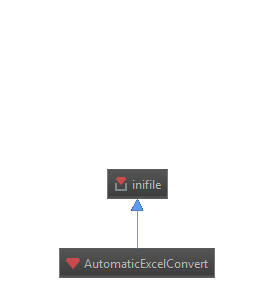
\includegraphics[scale=0.6]{pics/Gemdependency-full.png}
				\caption{Der Abhängigkeitsgraph der Gems}
				\label{Abhaengigkeitsgraph}
			\end{figure}
		\section{Gem einfügen}
			Das \robersexcelconvert-Gem muss um mit \sketchup funktionieren zu können in den richtigen Ordner kopiert werden. 
			Dazu muss der \glqq Plugins \grqq-Ordner geöffnet und die angegebene Datei und Ordner kopiert werden.
			Dies ist notwendig, damit das \robersexcelconvert-Gem direkt beim Start von \sketchup geladen wird und verwendet werden kann.
			\subsubsection{Plugins-Ordner}
				Der Plugins-Ordner ist erreichbar über die folgenden Schritte:
				\begin{enumerate}
					\item Windows Explorer öffnen:\\
						\begin{figure}[H]
							\centering
							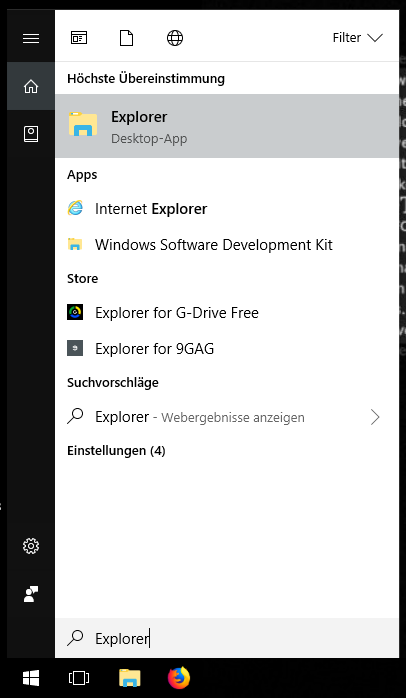
\includegraphics[scale=0.5]{pics/plugins-ordner/Explorer-oeffnen.png}
							\caption{Der Explorer wird mittels Starmenü geöffnet}
						\end{figure}
						Öffnen Sie den Explorer mittels des Windows-Startmenüs oder der Tastenkombination: \keystroke{Win}+\keystroke{E}
						\label{explorer oeffnen}
					\item Zur Roaming navigieren:\\
						\begin{figure}[H]
							\centering
							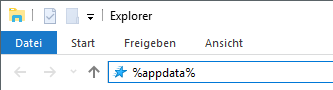
\includegraphics[scale=0.6]{pics/plugins-ordner/appdata-eingeben.png}
							\caption{In die Adresszeile wird die angegebene Text direkt eingefügt}
						\end{figure}						
						Navigieren Sie zur Roaming des Benutzers. Dies ist möglich durch die Eingabe von:\texttt{\%appdata\%} in die Adresszeile. Alternativ kann man den absoluten Pfad angeben, welcher meist wie folgt aussieht:
						\lstinputlisting[xleftmargin=0.1\textwidth,xrightmargin=0.2\textwidth]{listings/roamingpath.txt}
						wobei \texttt{BENUTZERNAME} durch den Namen des aktuellen Windows Nutzers ersetzt werden muss.\\
						\underline{Wichtig}: Es müssen versteckte Ordner angezeigt werden um manuell zum Roaming Ordner zu navigieren.
						\label{explorer oeffnen}
					\item Zum Plugins Ordner navigieren:
						\begin{figure}[H]
							\centering
							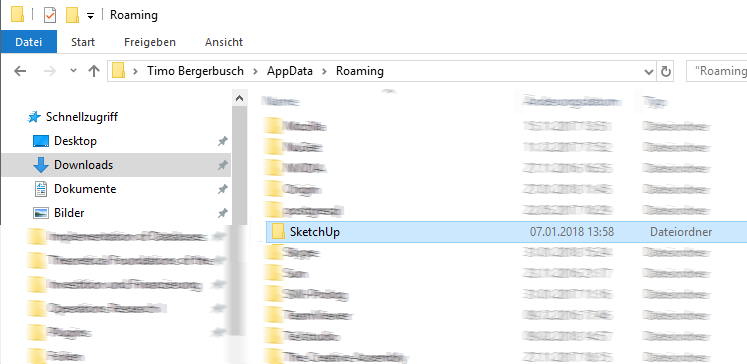
\includegraphics[scale=0.6]{pics/plugins-ordner/Sketchup-Ordner.png}
							\caption{Der \sketchup-Ordner in der Roaming}
						\end{figure}
						In dem nun geöffneten Roaming suche Sie nach dem Ordner mit Namen: \sketchup .
						Innerhalb von diesem Ordner öffnen Sie die folgende Ordnerstruktur: 
						\lstinputlisting[xleftmargin=0.1\textwidth,xrightmargin=0.2\textwidth]{listings/pluginspath.txt}
						Dies ist der Ordner in welchen nun mit dem folgenden Schritt das \robersexcelconvert-Gem eingefügt werden sollte.
					\item Kopieren:
						\begin{figure}[H]
							\centering
							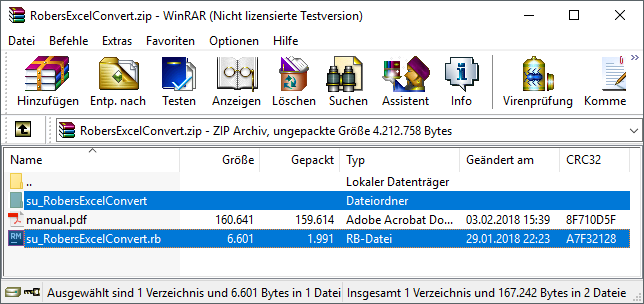
\includegraphics[scale=0.6]{pics/plugins-ordner/zip-datei.png}
							\caption{Die markierten zu kopierenden Datei und Ordner}
						\end{figure}
						Kopieren sie die markierten Datei \texttt{su\_RobersExcelConvert.rb} und den markierten Ordner \texttt{su\_RobersExcelConvert} in den soeben geöffneten \texttt{Plugins}-Ordner.
						\begin{figure}[H]
							\centering
							\includegraphics[scale=0.6]{pics/plugins-ordner/plugins-ordner.png}
							\caption{Der Plugins-Ordner nach dem einfügen der Datei und des Ordners}
						\end{figure}
				\end{enumerate}
		\section{Funktionstest}
			Wenn das \robersexcelconvert-Gem korrekt eingefügt wurde und das Gem wie gewünscht funktioniert kann per \hyperref[Ruby Konsole]{Ruby Konsole} getestet werden, ob das Plugin funktioniert\\
			Dazu muss in der Konsole der folgende Befehl eingegeben werden:
			\lstinputlisting[xleftmargin=0.2\textwidth,xrightmargin=0.2\textwidth]{listings/funktionstest.txt}
			Dies gibt bei korrekter Integration des Plugins: \texttt{true} zurück.\\
			Ansonsten wird ein Fehler zurück gegeben, dass die Methode nicht bekannt ist und somit das Plugin nicht richtig eingebunden wurde.
	\chapter{Excel-Datei}
		\section{Aufbau}
		\section{Anpassungsmöglichkeiten}
	\chapter{Bauteil Identifizierung}
		\section{Translations} \label{Translations}
			\subsection{Hinzufügen}
			\subsection{Aufbau}
			\subsection{Löschen}
	\chapter{Fehlerbehandlung}
		\section{Fehlercodes}
			\subsection*{Code: 0x00}
\end{document}